\documentclass{jsarticle}
\usepackage[dvipdfmx]{graphicx}
\begin{document}

\title{身体動作と筋電量の関係性}
\author{平松亨隆}
\maketitle


\section{目的}
私を含めて人は、意識的に筋肉の伸縮を考えて体を動かすわけではない。例えば、上腕二頭筋を使うことを意識して腕を曲げる人はまずいないだろう。だから、私達は運動の際に筋肉がどのように筋活動をしているのかを知らない。そこで今回は腕の曲げ伸ばし運動に着目して、上腕二頭筋と上腕三頭筋がどのような筋活動をしてその運動をしているのか、ということを本レポートの目的とした。

\section{実験方法}
\subsection{運動計測}
下記の図\ref{fig:short}はもっとも腕を曲げた状態、図\ref{fig:long}は最も腕を伸ばした状態の図である。被験者にはこの2つの状態を繰り返す腕の曲げ伸ばし運動を、利き腕を使って、速度に関して何も指示を出していない場合と速く動かしてもらった場合の2パターンで計測をした。被験者には反射マーカーを肩、肘、手首につけて。また筋電センサ(ロジカルプロダクト社)を上腕二頭筋と上腕三頭筋に貼付し、筋電位をサンプリング周波数は200 Hzで計測した。筋電センサとカメラの計測時間は同期をとり、20秒間計測していた。
\begin{figure}[h]
  \begin{minipage}{0.5\hsize}
    \begin{center}
      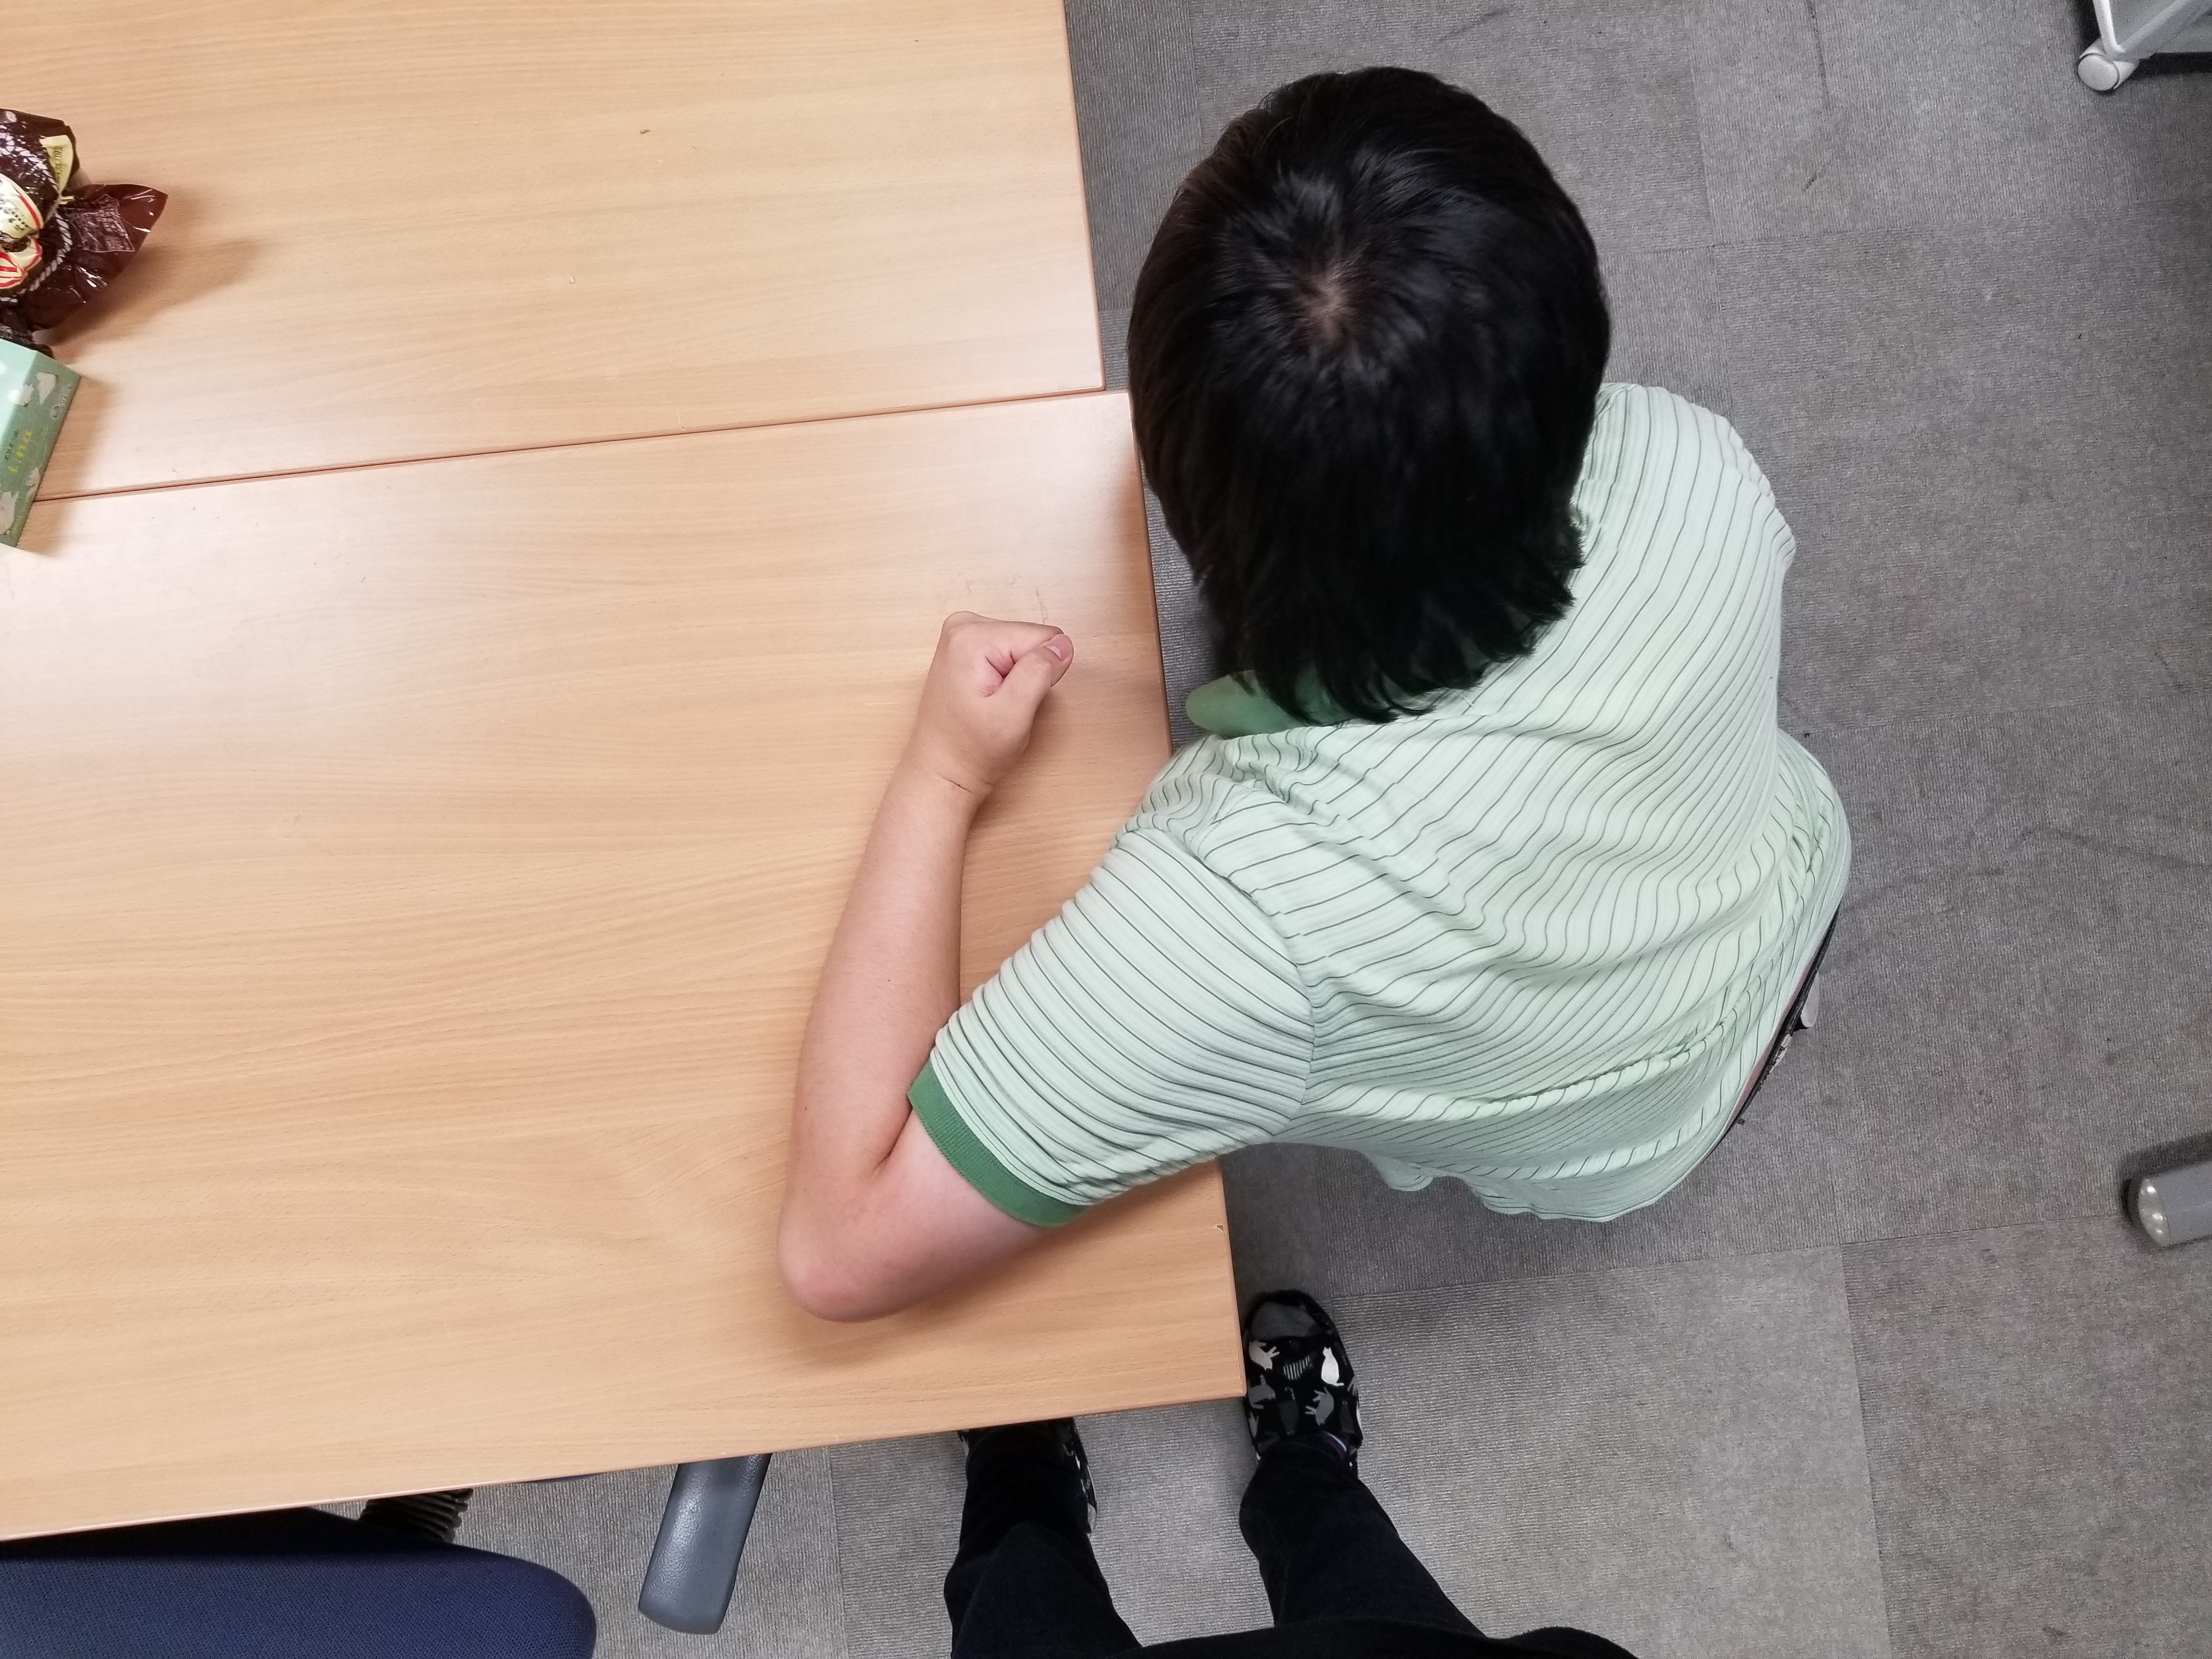
\includegraphics[width=7cm]{images/short.jpg}
    \end{center}
    \caption{腕を縮めた状態}
    \label{fig:short}
  \end{minipage}
  \begin{minipage}{0.5\hsize}
    \begin{center}
      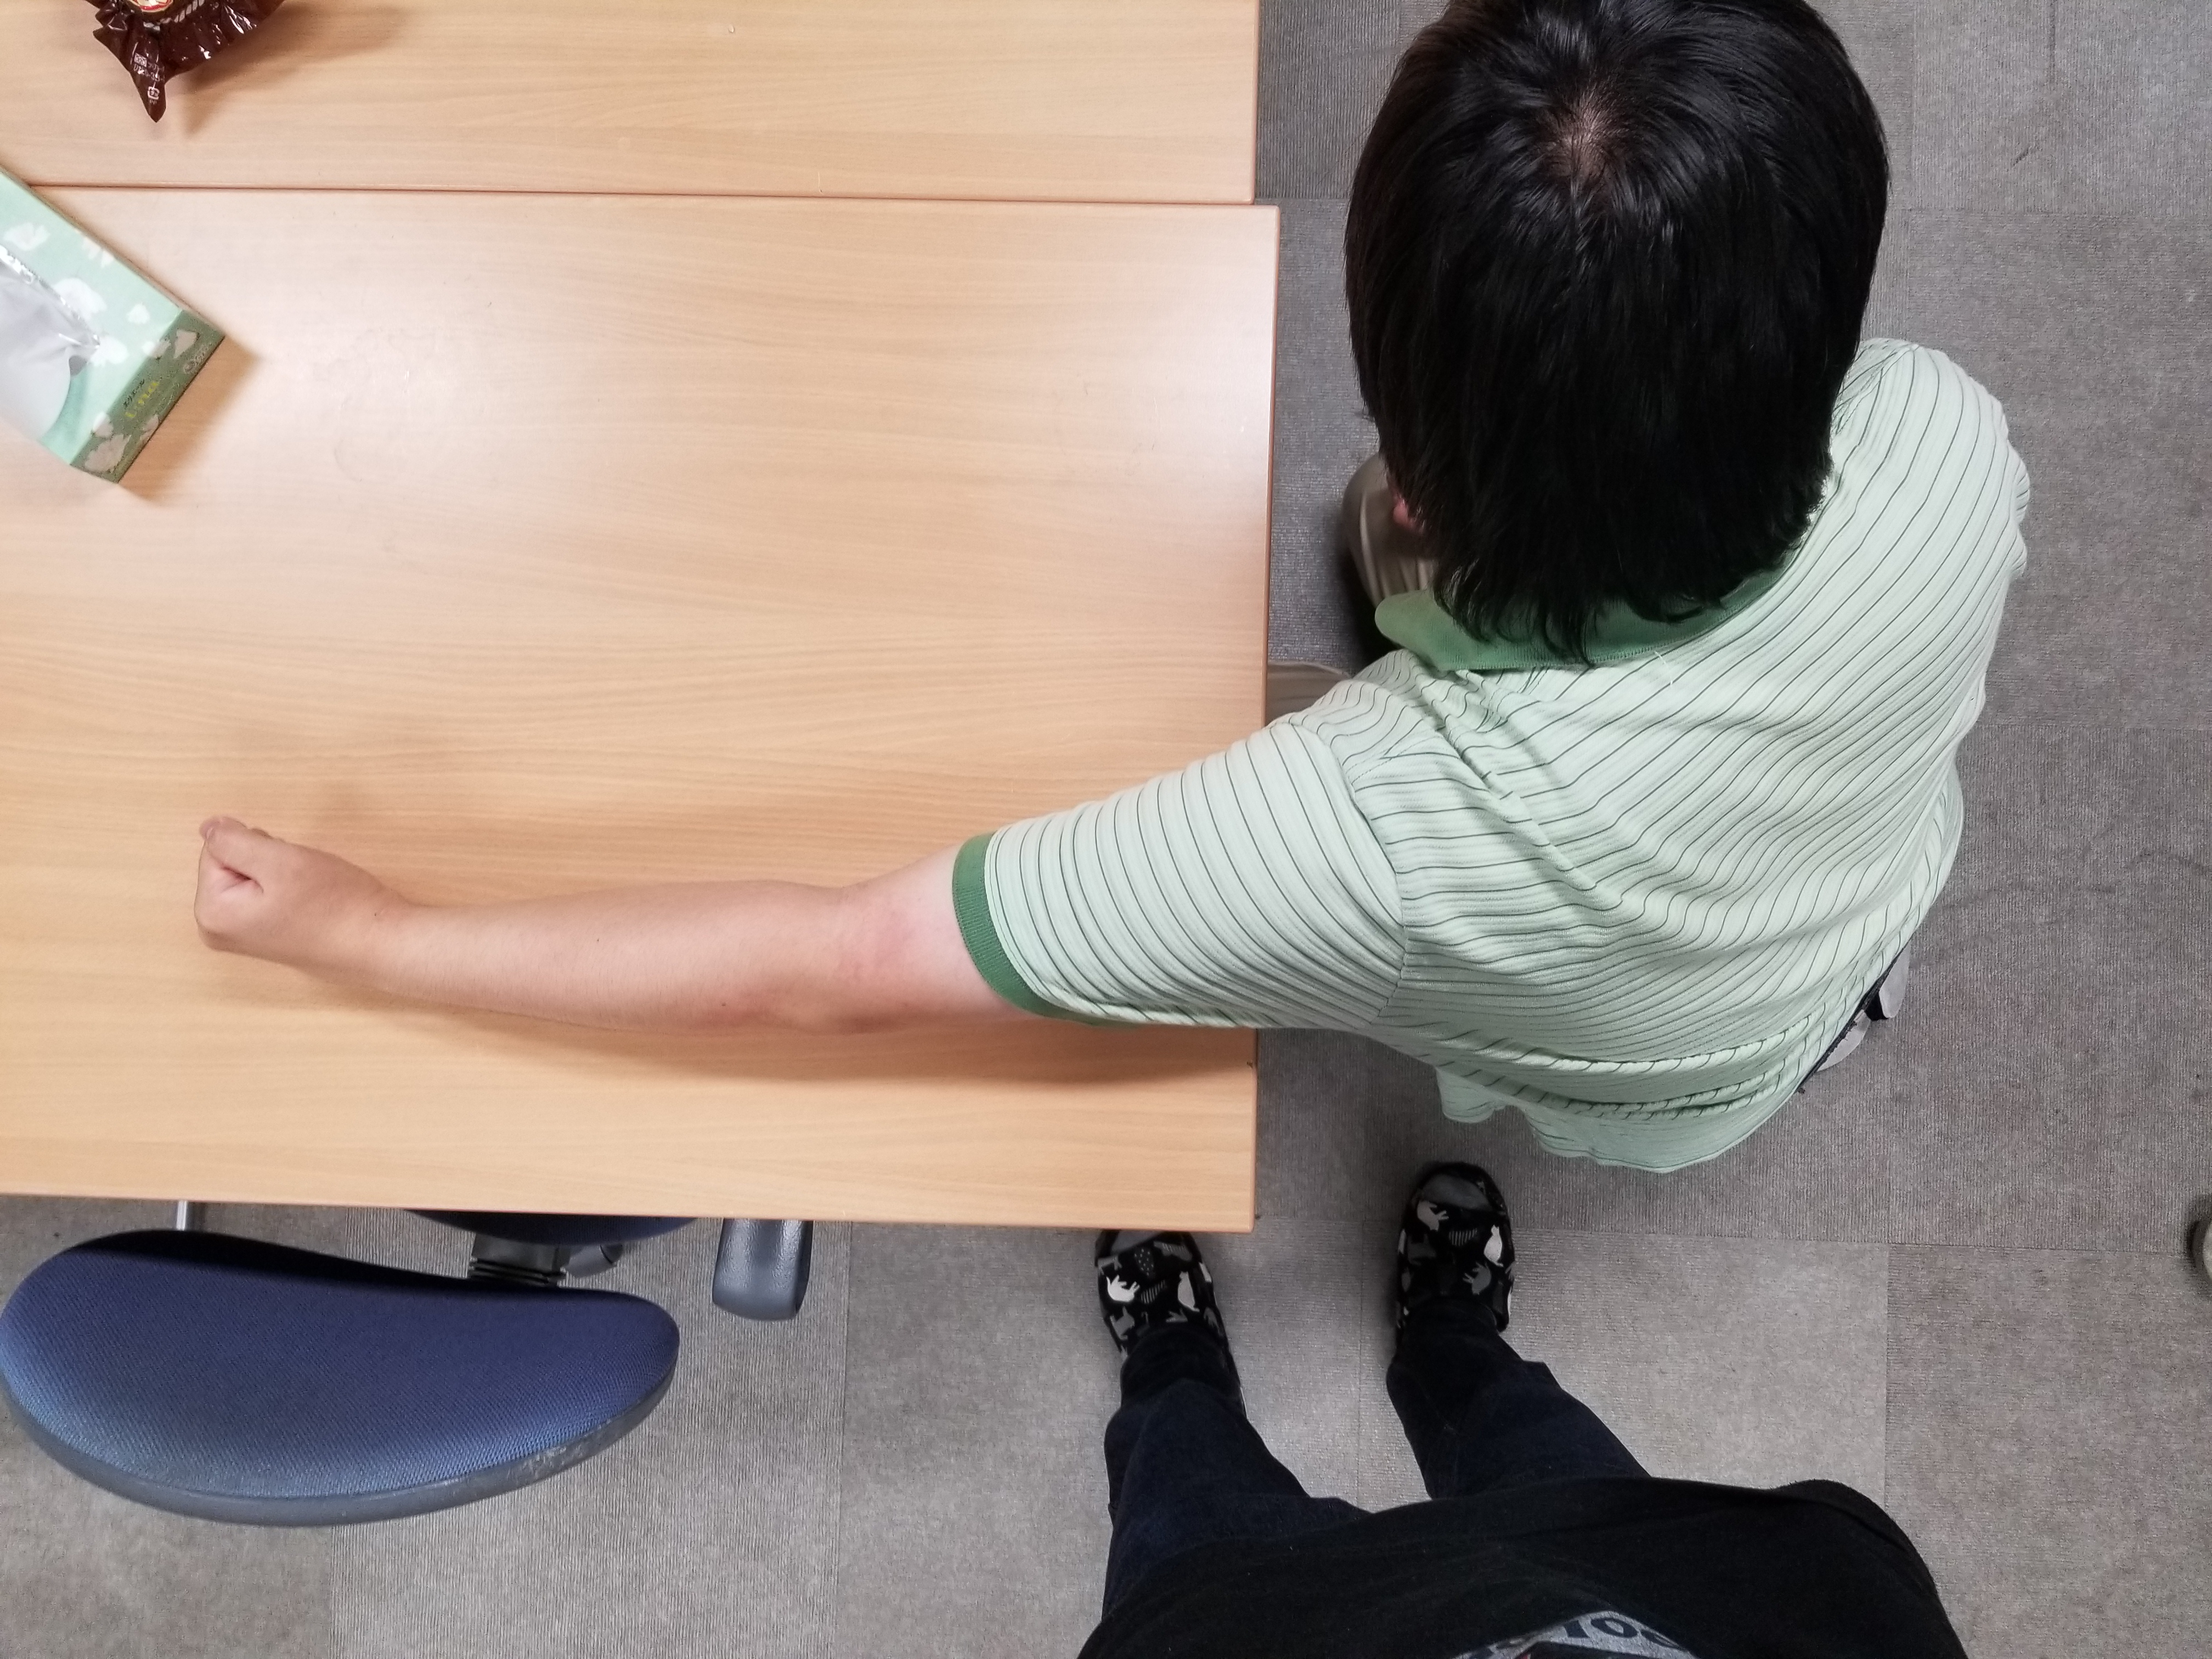
\includegraphics[width=7cm]{images/long.jpg}
    \end{center}
    \caption{腕を伸ばした状態}
    \label{fig:long}
  \end{minipage}
\end{figure}

\subsection{解析}
\subsubsection{筋電位}
筋電位のデータにはいくつかの処理を順番に施して、筋肉の活動度を求めた。
  まずデータから筋電位の特徴を抽出するために、通過帯域を1〜40 Hzとしたバンドパスフィルタ(3次バターワース)をかけた。しかし、バンドパスフィルタをかけることによってデータに位相ズレが生じるため、時間軸を反転してもう一度同じフィルタをかけることによってこれを補正した。そしてフィルタ後のデータを整流し、時刻$t$の筋電位$|E(t)|$に対して時間$\Delta T$の間で平均を求め、筋肉の活動度とした。式は以下を用いた。
  \begin{equation}
    a(t) = \frac{1}{\Delta T} \int_{t-\frac{\Delta T}{2}}^{t+\frac{\Delta T}{2}} |E(t)| dt
  \end{equation}

\section{結果}
\begin{figure}[b]
  \begin{center}
    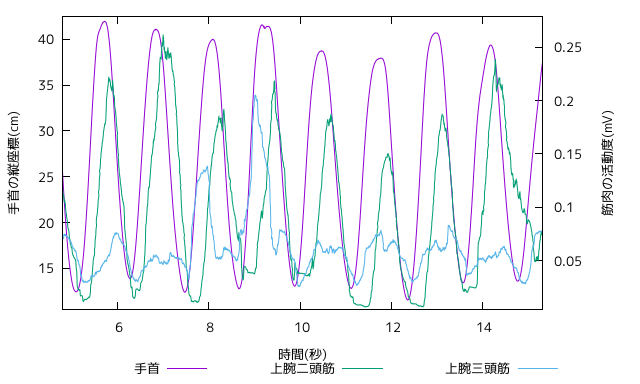
\includegraphics[width=15cm]{images/s1proto.png}
  \end{center}
  \caption{速度に関する指示のない運動と筋肉の活動度の関係}
  \label{fig:slow}
\end{figure}
図\ref{fig:slow}は、速度に関して指示を出さず腕を動かしてもらった場合である。身体に対する手首の前後方向の変位と筋肉の活動度を縦軸に、そして時間を横軸とした。このとき身体に対する手首の前後方向の変位は、体の前に伸ばすほど値は大きくなる。図中の紫、緑、青の線はそれぞれ身体に対する手首の前後方向の変位、上腕二頭筋肉の活動度、上腕三頭筋の活動度である。手首の前後方向の変位が、横方向や縦方向に比べて変位が大きく、動きが把握しやすい部分であったので抜き出した。このグラフでは、運動開始後時刻5〜15秒の間を表示している。

図\ref{fig:slow}から、例えば時刻10秒の時、腕がもっとも屈曲した状態であり、その後伸展を始め、少ししてから上腕二頭筋の活動度が大きくなっていっている。そして、伸ばしきったあとある程度腕を曲げたところでその活動度を下げはじめている。これはほとんどの場合において言えることである。またこの時上腕三頭筋は、最大値が上腕二頭筋よりもかなり小さいが、同じような挙動をしている。しかし、いくつかの例においては、腕を伸ばし始めてから伸ばしきるまでの間だけ、上腕二頭筋に匹敵する活動度を見せているものもある。

上腕二頭筋は使用頻度から上腕三頭筋よりも発達している。そのため、速度に関する指示を出していない場合で腕を伸展させるとき、上腕三頭筋は値として見れるほどの筋活動度を示していない可能性がある。逆に腕を屈曲させるとき、発達している上腕二頭筋が強い筋活動を行う。よって、腕が加速しすぎてしまうことを抑えるために上腕三頭筋は伸展させるときよりも強い筋活動を行う必要がある。以上のことにより、図\ref{fig:slow}のようになったのではないだろうか。

\begin{figure}[b]
  \begin{center}
    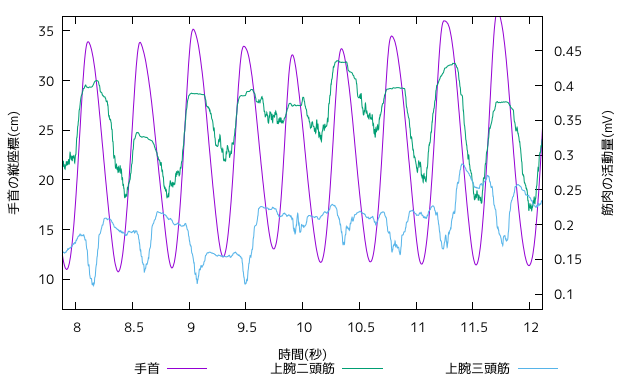
\includegraphics[width=15cm]{images/s2proto.png}
  \end{center}
  \caption{速い時の運動と筋肉の活動度の関係}
  \label{fig:fast}
\end{figure}
図\ref{fig:fast}は、腕を速く動かしてもらった場合である。各軸や凡例は図\ref{fig:slow}と同様である。このグラフでは、運動開始後時刻8〜12秒の間を表示している。図\ref{fig:fast}から、例えば時刻8.8秒の時、腕がもっとも屈曲した状態では上腕二頭筋の活動度は低い、この状態から腕が伸展を始めると同時に活動度が大きくなっていっている。また腕を屈曲するとともにその活動度を下げている。要するに手首の前後方向の変位と似たような形である。このとき上腕三頭筋は、腕をもっとも屈曲させた状態では活動度が大きく、腕が伸展させられるにしたがってその値が小さくなっていっている。これは、上腕二頭筋の逆位相のような形である。

腕を速く動かしてもらった場合、当然上腕二頭筋も上腕三頭筋も強い筋活動を求められるだろう。このとき腕を伸展させる場合、上腕三頭筋は腕を加速させるために働き、上腕二頭筋も加速した腕を減速、最終的に停止させる必要がある。このとき腕を屈曲させる場合、上腕二頭筋は腕を加速させるために働き、上腕三頭筋も加速した腕を減速、最終的に停止させる必要がある。そのため、図\ref{fig:fast}のようになっているのではないだろうか。

図\ref{fig:slow}と図\ref{fig:fast}を比較すると、速度に関する指示を出さない場合(図\ref{fig:slow})では上腕二頭筋と上腕三頭筋の活動度はほぼ同じ位相、速く動かしてもらった場合(図\ref{fig:fast})では逆位相となっている。

\section{考察}
上腕二頭筋と上腕三頭筋の活動度の速度による位相差がある理由は、上腕二頭筋と上腕三頭筋の発達の違いによるものが大きいと考えられる。速度に関する指示を出さなかった場合は筋肉をあまり使わない。しかし、腕を屈曲させる場合にのみ、発達している上腕二頭筋は働く。よって上腕三頭筋もこれの速度を抑える必要があるため、筋活動がデータに現れている。速く動かしてもらった場合はどちらの筋肉もよく使う。そのため、腕を屈曲させる場合には上腕三頭筋が加速、上腕二頭筋が抑制の役割を行う。また、腕を伸展させる場合には上腕二頭筋が加速、上腕三頭筋が抑制の役割を行う。よって上腕二頭筋と上腕三頭筋の筋活動度は逆位相のような関係になっている。

以上の考察から、速度に関する指示を出さなかった場合は、筋活動が微弱なためにデータにならず、腕を動かす際にどのように上腕二頭筋と上腕三頭筋が働いているのかということの参考にはなり得ない。そのため、腕を速く動かしてもらった場合が参考になると言えるだろう。つまり、腕を屈曲させる場合には上腕三頭筋が加速、上腕二頭筋が抑制の役割を行う。また、腕を伸展させる場合には上腕二頭筋が加速、上腕三頭筋が抑制の役割を行う。というように筋活動を行い、腕の屈伸運動をしているのだろう。
\end{document}